\documentclass[12pt]{article}
\usepackage{graphics}
\begin{document}

\noindent
Name:\,\makebox[0.8\textwidth]{\hrulefill} \\
\textbf{Observational Astronomy final exam} \\
2007 May \\
\resizebox{\textwidth}{!}{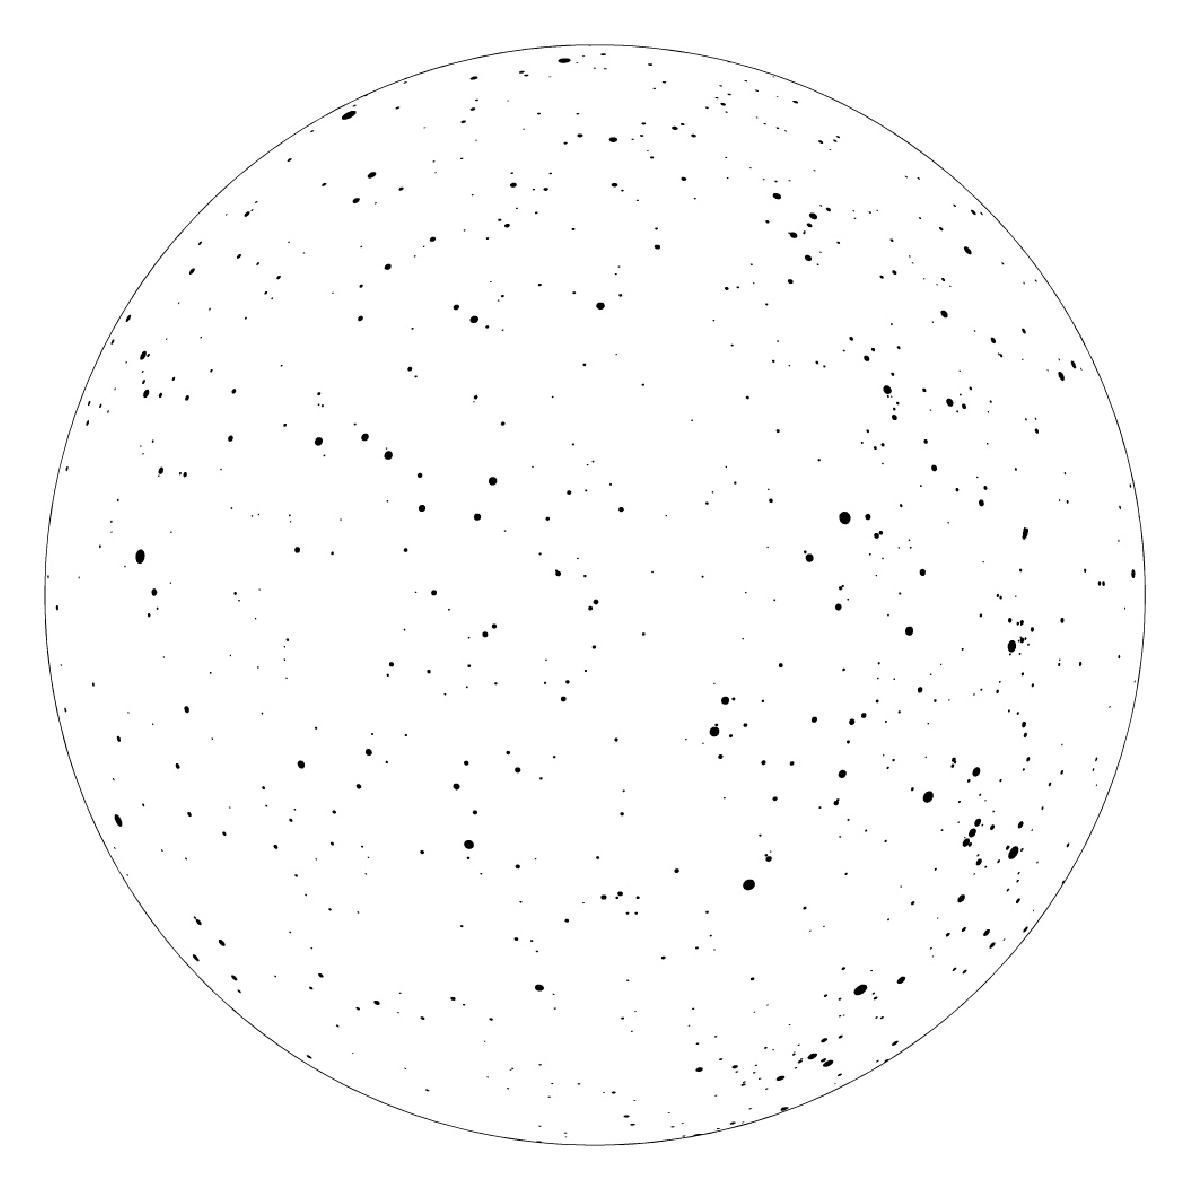
\includegraphics{final_chart.ps}}

\begin{enumerate}

\item (7 points)
Above is an unlabeled map of the sky with the NYC zenith at the
center, appropriate for some time tonight.  Perform each of the
requested actions, and clearly and carefully \emph{label} each of them
on the map:
\begin{itemize}
\item circle the Pleiades
\item circle Aldebaran
\item draw the location of Jupiter tonight
\item draw the location of Jupiter \emph{one year ago}
\item draw the location of the Moon \emph{the last time it was full}
\item draw the location of the Moon tonight
\item draw the location of Saturn tonight
\end{itemize}
Make sure each one is clearly labeled.  If any of these are not in the
map, clearly write ``not in map''.  \emph{Note that the map is
distorted at the edges; use your judgement.}

\item (2 points)
The circle around the outside of the map is the horizon.  Label the
points on the horizon directly N, E, S, and W and draw in the
meridian.  The zenith is in the center of the map.

\item (2 points)
To what sidereal time does the map correspond?

\vspace{0.5in}

\item (2 points)
On a spring night, which rises first, the Pleiades or Aldebaran?
Roughly what is the time difference between them?  Show your work.

\vspace{1in}

\item (2 points)
Which is brighter, Rigel or Sirius, and by what factor?  Show your
work.

\vspace{1in}

\item (1 point)
In NYC tonight, at what altitude does Aldebaran cross the meridian?

\vspace{0.5in}

\item (1 point)
In Equador (lat=$0$\,deg) tonight, at what altitude does
Aldebaran cross the meridian?

\vspace{0.5in}

\item (2 points)
According to sidereal time, Aldebaran crosses the meridian
earlier/later/at the same time compared to the previous night
(\emph{circle your answer}).

According to civil time, Aldebaran crosses the meridian
earlier/later/at the same time compared to the previous night.

\item (2 points)
Specify exactly the condition on the coordinates of a star that makes
it visible, at (at least) some moment during the year, for an observer
at latitude $\lambda$.

\vspace{1in}

\item (2 points)
Specify exactly the condition on the coordinates of a star (and, if
necessary, the latitude and the time of year) that makes it rise due
East and set due West.

\vspace{1in}

\item (2 points)
In NYC, you see a bright star near the horizon in the southwest.  You
re-observe the star 15\,min later, how has it moved?
\begin{itemize}
\item up and to the left
\item up and to the right
\item down and to the left
\item down and to the right
\end{itemize}

\item (1 point)
If the Sun is in the constellation Virgo (check the atlas), what is
the season?

\vspace{0.5in}

\item (2 points)
Give the date and time at which you started this exam.  What is the
sidereal time corresponding to that date and time?  Show your work.

\vspace{1in}

\item (2 points)
In NYC today, at what altitude did the Sun cross the meridian?
Describe your process for getting the answer.

\vspace{1in}

\item (2 points)
When (relative to sunrise, noon, sunset, or midnight) is a waning
crescent moon visible against a dark sky?  Which side is lit up?  Be
as specific as possible on both points.

\vspace{0.5in}

\item (2 points)
Describe a method in use today for the detection of extra-solar
planets.

\vspace{1in}

\item (1 point)
Why do some craters on the Moon look ``flooded''?

\vspace{1in}

\item (2 points)
What ``powers'' (provides the energy of) the Orion nebula?  Be as
specific as possible.

\vspace{1in}

\item (2 points)
Which way does a comet's tail point?

\vspace{1in}

\item (2 points)
Explain, briefly, what we get by pointing our telescopes at Polaris at
the beginning of the night.

\vspace{1in}

\item (3 points)
Give a very brief explanation of why it is possible to take a picture
with a cell-phone camera through the telescope on the roof without
adjusting the focus of either the telescope or the camera.

\vspace{1in}

\clearpage
\item (4 points)
This semester (Spring 2007) we did \emph{not} observe Jupiter's moons.
When (what year) is the next Spring semester in which we can
reasonably observe Jupiter's moons?  Show your work.

\emph{Hints:} Start by computing the sidereal time in the middle of
lab class in the middle of the first week of the semester and the same
for the last week of the semester.  That range of sidereal times is
somehow important.  We can observe things within a few hours of the
meridian.  That is also somehow important.  Look up Jupiter's future
motions on the sky in your Field Guide.  That is also somehow
important.

\vspace{2in}

\end{enumerate}
\end{document}
